\documentclass[11pt,letterpaper]{article}
\usepackage[margin=0.70in,top=0.72in,bottom=0.68in,headheight=14pt,headsep=14pt]{geometry}
\usepackage[T1]{fontenc}
\usepackage{lmodern,microtype,parskip,enumitem,amssymb}
\usepackage{tabularx,booktabs,array,xcolor,graphicx}
\usepackage{tikz}
\usetikzlibrary{arrows.meta,positioning,calc}
\usepackage{listings,fancyhdr,hyperref}
\definecolor{navy}{HTML}{15384A}
\definecolor{teal}{HTML}{007D82}
\definecolor{pale}{HTML}{EDF5F5}
\definecolor{ink}{HTML}{273742}
\definecolor{muted}{HTML}{536773}
\definecolor{line}{HTML}{CCD8DD}
\definecolor{amber}{HTML}{926300}
\definecolor{green}{HTML}{206642}
\definecolor{red}{HTML}{9A3232}
\hypersetup{colorlinks=true,urlcolor=teal,linkcolor=teal,pdfauthor={USF AI in FinTech course},pdftitle={Project 0: Payment Rails Live - Instructor Course Guide}}
\renewcommand{\familydefault}{\sfdefault}
\color{ink}
\setlength{\parindent}{0pt}
\setlength{\parskip}{5pt}
\setlength{\emergencystretch}{2em}
\setlist{nosep,leftmargin=16pt,topsep=5pt,itemsep=3pt}
\renewcommand{\arraystretch}{1.18}
\newcolumntype{Y}{>{\raggedright\arraybackslash}X}
\lstset{basicstyle=\ttfamily\fontsize{9}{11}\selectfont,columns=fullflexible,keepspaces=true,breaklines=true,showstringspaces=false,frame=single,rulecolor=\color{line},backgroundcolor=\color{pale},framesep=6pt,xleftmargin=6pt,xrightmargin=6pt,aboveskip=7pt,belowskip=7pt}
\pagestyle{fancy}\fancyhf{}
\fancyhead[L]{\fontsize{8.5}{10}\selectfont\color{muted}USF | AI in FinTech | Instructor demonstration}
\fancyhead[R]{\fontsize{8.5}{10}\selectfont\color{muted}Project 0}
\fancyfoot[L]{\fontsize{8}{10}\selectfont\color{muted}Payment Rails Live | Fictional USD debit-card flow}
\fancyfoot[R]{\fontsize{8}{10}\selectfont\color{muted}\thepage\ / 10}
\renewcommand{\headrulewidth}{0.3pt}
\newcommand{\pagetitle}[2]{\noindent{\color{teal}\small\bfseries #1}\par\vspace{2pt}{\color{navy}\fontsize{21}{24}\selectfont\bfseries #2}\par\vspace{7pt}}
\newcommand{\smalltitle}[1]{\par\vspace{5pt}{\color{navy}\large\bfseries #1}\par\vspace{2pt}}
\newcommand{\screen}[2]{\begin{center}\IfFileExists{../screenshots/#1}{\includegraphics[width=\linewidth,trim=0 180bp 0 450bp,clip]{../screenshots/#1}}{\fcolorbox{line}{pale}{\parbox[c][#2][c]{0.94\linewidth}{\centering\textbf{Screenshot asset: #1}\par The full distribution includes the captured running dashboard in the screenshots folder. A standalone editor preview can omit external image assets.}}}\end{center}}
\begin{document}
\pagetitle{01 / INSTRUCTOR GUIDE}{Payment Rails Live}
{\color{navy}\Large\bfseries Watch a card payment travel through six programs}\par
USF AI in FinTech | Project 0 | Instructor demonstration

\smalltitle{Why start here?}
A payment approval is a decision. It does not mean the merchant has already received the sale proceeds. This demonstration makes the decisions, messages, temporary holds, and later financial effects visible, one message at a time.

Six small Python processes represent the payer, merchant/POS, gateway/processor, acquirer, simulated Visa or Mastercard network, and issuer. An animated browser dashboard follows actual messages from those processes. The programs use deterministic rules; no language model chooses whether a payment succeeds.

\begin{quote}\textbf{The classroom question}\par
A payer has \$500. A merchant requests \$50. When the POS says Approved, where is the money? Show the hold, capture the payment, clear the batch, then settle it. Explain why the merchant receives \$48.75.\end{quote}

\smalltitle{What the audience will observe}
\begin{itemize}
\item The request travels forward; the issuer's decision travels back through every participant.
\item Authorization reserves \$50: posted balance remains \$500; available balance becomes \$450.
\item Capture records the merchant's intent to collect. Clearing posts a \$50 debit in this toy model.
\item Settlement credits \$48.75 to the merchant and \$1.25 to illustrative fee allocations.
\item A decline, a duplicate, and an invalid transition produce visible reasons without inventing money movement.
\end{itemize}

\smalltitle{Use the delivered implementation}
Start the project, project the dashboard, and run the script on pages 7--8. The package contains working source, fictional fixtures, automated tests, editable diagrams, two PDFs with LaTeX sources, screenshots, and a verification record. This is an unscored instructor example, with an observation checklist rather than a submission requirement.

\smalltitle{Teaching boundaries}
One USD debit-card flow, one instructor session, full capture, temporary memory, and accelerated batches keep the implementation small. No real cards, bank connections, model API, refunds, chargebacks, partial capture, or crash recovery are included. Debit posting at clearing is a teaching convention; real scheme and issuer timing varies.

\clearpage
\pagetitle{02 / INSTRUCTOR GUIDE}{Six actors, six responsibilities}
The six boxes are distinct running programs. In real commerce, a single provider can bundle several roles. The separation here makes the responsibilities easier to see.

\begin{tabularx}{\linewidth}{>{\raggedright\arraybackslash}p{3.7cm}Y}
\toprule
\textbf{Actor} & \textbf{What its program demonstrates} \\ \midrule
Payer & Starts a fictional purchase and receives its final outcome. The issuer owns the authoritative account balance. \\
Merchant / POS & Accepts the purchase, sends the authorization request, records the returned decision, and initiates full capture. \\
Gateway / processor & Checks the request contract, preserves identifiers, and routes valid payment operations. \\
Acquirer & Represents the merchant side, tracks authorized/cleared records, and records merchant proceeds plus illustrative fee allocations. \\
Simulated card network & Routes Visa or Mastercard messages, checks batch membership and totals, and validates batch membership and totals. \\
Issuer & Looks up the synthetic account, checks account status and available funds, owns holds and posted balances, and processes clearing/settlement obligations. \\
\bottomrule
\end{tabularx}

\smalltitle{Three words to distinguish}
\begin{tabularx}{\linewidth}{>{\raggedright\arraybackslash}p{3.7cm}Y}
\toprule
\textbf{Word} & \textbf{Meaning in this demonstration} \\ \midrule
Message & A request or response that one actor sends to another. Message animation represents communication. \\
State & What an actor currently remembers: an authorization, hold, capture, balance, batch, or fee allocation. \\
Agent & A small program with a role, local state, and rules for handling incoming messages. It does not require AI or an LLM. \\
\bottomrule
\end{tabularx}

\smalltitle{Narration to use at the diagram}
``The merchant asks for permission. The issuer makes the account decision. The network carries that decision; the acquirer connects the merchant side. Later, the approved sale becomes a claim for payment and is settled.''

A gateway is especially visible in online payments. A physical POS can connect through different processor arrangements. Project 0 deliberately uses the same six-hop route for every purchase so the audience can follow one consistent example.

\smalltitle{Evidence to point to}
Each card on the dashboard shows its process ID and latest activity. A message record shows sender, recipient, payment ID, operation ID, amount, and outcome. The PID is evidence that a role is running separately; the trace is evidence of what it actually handled.

\clearpage
\pagetitle{03 / INSTRUCTOR GUIDE}{Architecture you can point to}
\begin{center}
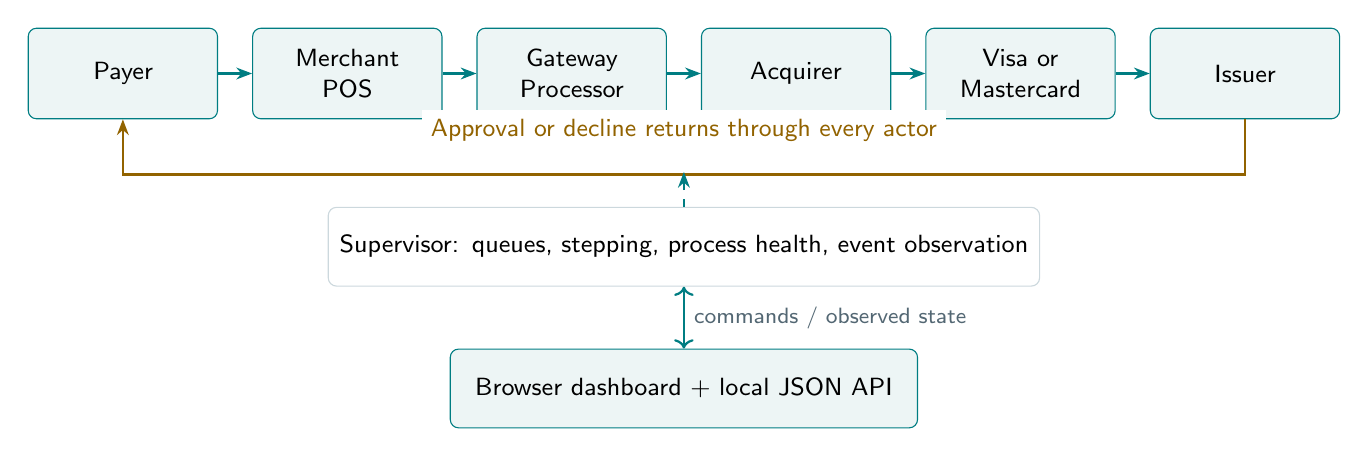
\begin{tikzpicture}[font=\fontsize{9}{11}\selectfont,box/.style={draw=teal,fill=pale,rounded corners=3pt,align=center,text width=2.17cm,minimum height=1.15cm},arr/.style={-{Stealth[length=2mm]},thick,teal}]
\foreach \name/\label/\x in {p/Payer/0,m/{Merchant\\POS}/2.85,g/{Gateway\\Processor}/5.7,a/Acquirer/8.55,n/{Visa or\\Mastercard}/11.4,i/Issuer/14.25}{\node[box] (\name) at (\x,0) {\label};}
\draw[arr] (p)--(m);\draw[arr] (m)--(g);\draw[arr] (g)--(a);\draw[arr] (a)--(n);\draw[arr] (n)--(i);
\draw[arr,draw=amber] (i.south)--++(0,-0.7)-|(p.south);
\node[text=amber,fill=white,align=center] at (7.125,-0.72) {Approval or decline returns through every actor};
\node[draw=line,fill=white,rounded corners=3pt,align=center,text width=8.8cm,minimum height=1.0cm] (s) at (7.125,-2.2) {Supervisor: queues, stepping, process health, event observation};
\draw[arr,dashed] (s.north)--(7.125,-1.25);
\node[box,text width=5.7cm,minimum height=1.0cm] (b) at (7.125,-4) {Browser dashboard + local JSON API};
\draw[arr,<->] (s)-- node[right,text=muted,font=\fontsize{8.5}{10}\selectfont]{commands / observed state} (b);
\end{tikzpicture}
\end{center}

\smalltitle{What starts with one command}
The parent Python program starts six child processes, then serves bundled HTML, CSS, and JavaScript at \url{http://127.0.0.1:8010}. Each role has an inbox queue. The supervisor delivers the next queued message and collects the resulting events and state snapshots.

The supervisor controls pacing and displays observations. It does not approve transactions or manufacture balances. Those rules and balances belong to participant programs.

\smalltitle{Read the diagram in two directions}
The top path carries an authorization request toward the issuer. The lower return path carries the issuer's result back to the payer. Capture is a local merchant operation. Clearing and settlement travel from merchant through gateway, acquirer, and network to issuer, then return to merchant.

\smalltitle{Why this is a useful minimal implementation}
\begin{itemize}
\item Local queues avoid account setup, network services, and paid APIs.
\item Separate processes show the boundary between transport and participant decisions.
\item A shared event stream connects console evidence to the browser animation.
\item Source diagrams in \texttt{docs/diagrams} can be edited as Mermaid; SVG exports can be inserted into slides.
\end{itemize}

\clearpage
\pagetitle{04 / INSTRUCTOR GUIDE}{Follow one \$50 purchase}
Start from Reset. Use the approved preset and remain in Guided mode. Advance messages until the transaction reaches the stage named below; a button click can enqueue work before the final response returns.

\begin{tabularx}{\linewidth}{>{\raggedright\arraybackslash}p{2.7cm}>{\raggedright\arraybackslash}p{3.0cm}Y}
\toprule
\textbf{Stage} & \textbf{Instructor action} & \textbf{What the audience should see} \\ \midrule
Authorization & Create purchase; Next Message repeatedly & Forward request, issuer checks, reverse approval. Posted \$500; hold \$50; available \$450. \\
Capture & Select payment; Capture; advance & Merchant confirms full \$50 collection. The hold remains. No merchant proceeds yet. \\
Clearing & Clear Batch; advance & Captured sale is validated; issuer releases the hold and posts \$50. Posted \$450; held \$0; obligation \$50. \\
Settlement & Settle Batch; advance & Cleared batch membership/amounts reconcile. Obligation becomes \$0; merchant receives \$48.75. \\
\bottomrule
\end{tabularx}

\smalltitle{The visible account arithmetic}
\begin{center}
\begin{tikzpicture}[font=\small,box/.style={draw=teal,fill=pale,rounded corners=3pt,align=center,text width=4.2cm,minimum height=1.2cm},arr/.style={-{Stealth},thick,teal}]
\node[box] (a) at (0,0) {Before purchase\\Posted \$500 / Held \$0\\Available \$500};
\node[box] (b) at (5.5,0) {Authorized + captured\\Posted \$500 / Held \$50\\Available \$450};
\node[box] (c) at (11,0) {Cleared + settled\\Posted \$450 / Held \$0\\Available \$450};
\draw[arr] (a)--(b);\draw[arr] (b)--(c);
\end{tikzpicture}
\end{center}
Available funds equal posted balance minus active holds. After clearing, available funds stay \$450: a hold has been replaced by a posted debit, not charged a second time.

\smalltitle{Where \$1.25 goes in the toy fee policy}
\begin{tabularx}{\linewidth}{Yrr}
\toprule
\textbf{Allocation} & \textbf{Policy} & \textbf{\$50 example} \\ \midrule
Issuer interchange & 2\% & \$1.00 \\
Network fee & 0.1\% & \$0.05 \\
Processor/acquirer fee & 0.2\% + \$0.10 & \$0.20 \\
Merchant proceeds & Gross less all fees & \$48.75 \\ \bottomrule
\end{tabularx}
These rates are invented for arithmetic clarity. They are not Visa, Mastercard, Stripe, or any bank's price list. Integer-cent components are rounded separately, half up. The toy rejects a purchase if its configured fees exceed its amount.

\clearpage
\pagetitle{05 / INSTRUCTOR GUIDE}{Start the local demonstration}
\smalltitle{Requirements}
Use Python 3.9 or later and a current browser. The runtime uses Python's standard library and bundled assets. No pip install, cloud account, card credentials, or model API key is needed. Purchases use integer cents from 100 through 1000000 (\$1--\$10,000).

Unzip the full package and keep its directory structure. Open a terminal in \texttt{project-0-payment-rails}. Run:
\begin{lstlisting}
python3 start.py
\end{lstlisting}
On Windows PowerShell use:
\begin{lstlisting}
py -3 start.py
\end{lstlisting}
The delivered launchers provide an alternative to typing the command. The README names them and lists options. A terminal remains visible with role IDs and readable message logs. Keep that terminal open throughout the demonstration.

\smalltitle{Before students enter the room}
\begin{enumerate}
\item Open \url{http://127.0.0.1:8010}. Confirm six participant cards report running process IDs.
\item Choose Guided mode and reset. Start the approved preset and advance a few messages.
\item Check that the highlight follows the trace. Reset again for the class opening.
\item Set browser zoom for the projector. Use a wide screen so all six actors remain easy to follow.
\end{enumerate}

\smalltitle{Stop and restart}
Press Ctrl+C in the launch terminal. The supervisor shuts down the server and child processes. Relaunching starts fresh fictional accounts and history. Reset also restarts all participants together; browser refresh alone is not a financial reset.

\smalltitle{If port 8010 is already occupied}
Stop your prior demonstration or choose another local port:
\begin{lstlisting}
python3 start.py --port 8011 --no-browser
\end{lstlisting}
Open \url{http://127.0.0.1:8011}. The browser uses relative API paths, so it follows the chosen port.

\smalltitle{Container and cloud path}
Python is the lowest-friction classroom route. The Dockerfile packages the same application. The technical supplement gives local container commands and VM/SSH-tunnel paths for AWS, GCP, and Azure. Those are deployment instructions, not claims that cloud resources have been provisioned.

\clearpage
\pagetitle{06 / INSTRUCTOR GUIDE}{Screens from the running dashboard}
\textbf{A. Approved authorization.} These are detail crops of the delivered running application. Full captures are included in the screenshots folder; PIDs and timestamps vary.
\screen{approved.png}{2.22in}
Explain the forward request and reverse response. Point to the issuer's hold, the payer's available balance, and the selected message's payment ID.

\textbf{B. Declined authorization.} Reset, choose insufficient funds, and advance to the returned decline.
\screen{declined.png}{2.22in}
The reason should be visible along with the unchanged balances. A declined response is a completed issuer decision, not a missing message or a server fault.

The full captures also show the controls and message inspector. The financial panels above are participant state, not an animation-only illustration.

\clearpage
\pagetitle{07 / INSTRUCTOR GUIDE}{An eight-minute demonstration}
\begin{tabularx}{\linewidth}{>{\raggedright\arraybackslash}p{1.5cm}>{\raggedright\arraybackslash}p{4.0cm}Y}
\toprule
\textbf{Time} & \textbf{Action} & \textbf{Say / observe} \\ \midrule
0:00 & Reset; point to six actors & Each role is a separate Python process. Find the payer's \$500 opening balance. \\
0:45 & Approved purchase; step & Follow who receives each message. The issuer is the account decision-maker. \\
2:00 & Finish reverse response & Approval creates a hold. Posted balance is still \$500. \\
3:00 & Capture; advance & The merchant is now requesting collection of the approved sale. \\
4:00 & Clear Batch; advance & A posted debit replaces the hold; an unsettled obligation remains. \\
5:00 & Settle Batch; advance & Merchant proceeds are \$48.75. Show the three fee components and the \$50 total. \\
6:15 & Replay the operation & Inspect duplicate evidence. Explain why the same operation must not debit twice. \\
7:00 & Reset; insufficient preset & Advance to the decline, then identify the reason and unchanged funds. \\
\bottomrule
\end{tabularx}
\screen{settled.png}{2.25in}
\textbf{Settlement screenshot.} The running app shows the settled payment and merchant/fee allocations. The diagram's moving message is communication evidence; the ledger values are financial-state evidence.

\smalltitle{Three audience prompts}
\begin{enumerate}
\item At approval, which value changed: posted balance, held funds, or merchant proceeds?
\item After clearing, why did available funds not drop by another \$50?
\item Why does retrying the same operation produce evidence rather than another debit?
\end{enumerate}

\clearpage
\pagetitle{08 / INSTRUCTOR GUIDE}{Inspect messages and exceptions}
Select one transaction, then select a message in its event history. Read the plain-English explanation first. Expand the JSON to connect the explanation to the actual fields.

\begin{lstlisting}
{
  "payment_id": "P0001",
  "operation_id": "P0001:authorize",
  "sender": "network", "recipient": "issuer",
  "type": "AUTHORIZE",
  "amount_cents": 5000, "currency": "USD",
  "outcome": "", "reason": ""
}
\end{lstlisting}
These are actual envelope field names; this abbreviated example omits the synthetic account, merchant, brand, and session metadata. Export the actual JSON trace to see exact values from your run. Preserve IDs across hops; sender and recipient change as the message travels.

\smalltitle{Four useful comparison cases}
\begin{tabularx}{\linewidth}{>{\raggedright\arraybackslash}p{3.8cm}Y}
\toprule
\textbf{Case} & \textbf{What to demonstrate} \\ \midrule
Insufficient funds & Valid active account; request exceeds available funds. Decline returns through the same path; no hold is added. \\
Inactive account & Account exists but cannot authorize. Compare the reason with insufficient funds. \\
Invalid account / input & Unknown synthetic token or invalid amount/currency is rejected visibly. Contract rejection can occur before the issuer. \\
Repeated operation & Replay preserves the operation identity. The recorded response is returned with no additional financial change. \\
\bottomrule
\end{tabularx}

\smalltitle{Operations are ordered}
Capture requires authorization. Clearing requires capture. Settlement requires a reconciled cleared batch. Pressing a later-stage control too early must expose a reason and leave funds unchanged. Wait until the queued response completes before narrating a stage as finished.

\smalltitle{Automatic mode as a closing demonstration}
Reset with the default seed. Start Automatic and adjust the speed. Watch both approvals and declines, with capture/clearing/settlement accelerated into seconds. Pause to inspect a payment. Use keyboard focus and shortcut hints; reduced motion preserves readable highlights while disabling travel animation. The random input sequence repeats with the same seed; process IDs and wall-clock timing do not.

\clearpage
\pagetitle{09 / INSTRUCTOR GUIDE}{Observation checklist and troubleshooting}
\smalltitle{Unscored instructor observation checklist}
\begin{itemize}
\item[$\square$] Six different participant process IDs are visible and running.
\item[$\square$] A request crosses all six actors, and an issuer result returns through every actor.
\item[$\square$] Authorization adds a hold without lowering posted balance.
\item[$\square$] Capture keeps the hold; clearing posts exactly one debit and releases it.
\item[$\square$] Settlement removes the obligation and shows proceeds plus fees equal gross.
\item[$\square$] Declines show a reason; replay leaves funds unchanged.
\item[$\square$] A JSON trace matches the animated hop and displayed transaction.
\item[$\square$] Reset clears the history and replaces all participant processes.
\end{itemize}

\smalltitle{Resolve a classroom interruption}
\begin{tabularx}{\linewidth}{>{\raggedright\arraybackslash}p{4cm}Y}
\toprule
\textbf{Symptom} & \textbf{Next action} \\ \midrule
Python command missing & Try \texttt{py -3} on Windows or install Python 3.9+. Check the README's prerequisite command. \\
Browser did not open & Keep the terminal running; manually open the printed local URL. \\
Address already in use & Stop an earlier run or launch with \texttt{--port 8011}. \\
Nothing moves in Guided & Press Next Message. Guided queues wait for instructor delivery. \\
Automatic has stopped & Check Pause, participant health, and terminal logs; select a slower speed to inspect. \\
Worker failure shown & Preserve the trace if useful, then Reset. The toy pauses rather than making up a response. \\
Unexpected state after refresh & Refresh observes the same supervisor session. Use Reset for fresh accounts. \\
Tiny projected text & Increase browser zoom and use a wide window. Read the selected message panel aloud. \\
\bottomrule
\end{tabularx}

\smalltitle{What a failure means here}
A crashed participant is different from a declined payment. A decline is a valid business result; a crash prevents the process from answering. The application marks the failure, pauses, and requires Reset. There is no promise of recovering financial state after a process or machine crash.

\clearpage
\pagetitle{10 / INSTRUCTOR GUIDE}{Artifacts, next steps, and sources}
\smalltitle{What is in Project 0}
\begin{tabularx}{\linewidth}{>{\raggedright\arraybackslash}p{4.2cm}Y}
\toprule
\textbf{Artifact} & \textbf{Purpose} \\ \midrule
Runtime + browser assets & One-command, six-process demonstration with live events and balances. \\
Fictional fixtures + tests & Reproducible accounts/scenarios and financial/operation acceptance checks. \\
README + launchers & Quick start, controls, API examples, shutdown, and container instructions. \\
Course guide + LaTeX & This 10-page instructor walkthrough in PDF and editable source. \\
Technical design + LaTeX & Message/state rules, architecture, failure behavior, tests, and cloud evolution. \\
Mermaid + SVG diagrams & Architecture, authorization sequence, lifecycle, cloud evolution; editable and slide-ready. \\
Actual screenshots & Approval, decline, and settlement from the delivered running app. \\
AI-use + verification record & Generated-work provenance and checks that actually ran, with limitations. \\
Manifest + ZIP & File inventory and a portable full-source distribution. \\
\bottomrule
\end{tabularx}

\smalltitle{A forward path without changing the lesson}
Keep the local program for the first demonstration. Containerize the same six processes next. For a cloud classroom session, run the container on one Linux VM and open it through an SSH tunnel. Only later replace local queues with managed messaging and add durable state, authentication, and independently deployed participants. The supplement separates the working package from that future design.

\smalltitle{Reading and provenance}
\begin{itemize}
\item Adnan Masood, PhD., \emph{Agentic Payments 101 (1/2): How the Card Payment System Works}, July 11, 2026. User-supplied article excerpt; conceptual teaching context.
\item \href{https://developer.visa.com/capabilities/visanet-connect-acceptance/docs}{VisaNet Connect -- Acceptance: getting started}. Primary documentation for authorization/capture and issuer-response routing.
\item \href{https://developer.visa.com/pages/glossary}{Visa developer glossary}. Definitions of issuer, acquirer, authorization, clearing, and settlement.
\item \href{https://docs.stripe.com/payments/place-a-hold-on-a-payment-method}{Stripe: Place a hold on a payment method}. Primary documentation illustrating separate authorization and capture.
\end{itemize}
Sources checked October 6, 2026. Project 0's fee rates, queue transport, explicit stepping, and clearing-time debit are teaching choices. The simulated Visa/Mastercard box has no connection to either network.
\end{document}
